\documentclass{article}

\usepackage{amsmath}
\usepackage{graphicx}
\usepackage{float}

\usepackage{biblatex}
\usepackage{listings}

\usepackage{subcaption}
\usepackage{algorithm}
\usepackage{clrscode3e}

\lstset{
	numbers=left,
	numbersep=5pt,
	columns=fixed,
	breaklines=true
}

\addbibresource{INF250.bib}

\title{Non-stop and where to find them}
\author{Mats Hoem Olsen}
\date{2/11-2021}

\begin{document}
\maketitle
\tableofcontents
\listofalgorithms
\newpage
\section{Information about the picture}
We can tell from the picture we were given that the camera used had the following properties:
\begin{enumerate}
\item Canon EOS 5D Mark II
\item firmware version 2.0.8
\item Automatic exposure
\item Canon EF 28-70mm f/2.8L USM lens
\item aperture in the range 3 to 32
\item the camera had an average temperature of 27c
\item focal length 52mm
\item colour space is "sRGB"
\item the picture was taken as 2/11/2011 at 15:22:27.
\end{enumerate}

\section{The theory of my approach}

This section is divided into several progresses to handle the problem of the invisible Non-stops.

\subsection{Grayscale}

The formula used to calculate the grayscale of the image is:
$$
\text{pixel}=\min(Green,Blue,Red)
$$

\subsection{Opening}[H]
To perform the “opening” operation, we will use the following algorithm\cite[page:185-186,192]{wilhelm_burger_digital_nodate}
\begin{algorithm}[H]
\caption{Opening procedure}
\begin{codebox}
\Procname{$\proc{Opening}(A,H):$}
\li \Return $\proc{Dilate}(\proc{Erode}(A,H),H)$
\end{codebox}
\end{algorithm}
These algorithms are written as follows:

\begin{algorithm}[H]
\caption{Dilate procedure}
\begin{codebox}
\Procname{$\proc{Dilate(A,H)}:$}
\li Create map $A'$: $M\times N \to \{0,1\}$
\li \For $(p)\in M\times N$
\li \Do $A'(p)\gets 0$
\End
\li \For $(q)\in H$
\li \Do \For $(p)\in A$
\li \Do $A'(p+q) \gets 1$
\End
\End 
\li \Return $A'$
\end{codebox}
\end{algorithm}
The Erode procedure as its own algorithm however it can be expressed as a extension of dilation.
\begin{algorithm}[H]
\caption{Erode procedure}
\begin{codebox}
\Procname{$\proc{Erode(A,H)}:$}
\li $\bar{I}\gets \proc{Invert}(A)$
\li $H^*\gets \proc{Reflect}(H)$
\li $I'\gets \proc{Invert}(\proc{Dilate}(\bar{I},H^*))$
\li \Return $I'$
\end{codebox}
\end{algorithm}

These will help us to remove noise from our picture, given a sutible sized H. This is to make sure that when we proceed we will not get small areas of interest that is not sutible.

\subsection{Watershed}\label{sec:watershed}
Watersheding is not a spesific algorithm but rather a idea of how to segment a blob\cite{noauthor_watershed_2012}. The following is a prosegure of my own design\footnote{If it is an replication of another known algorithm, then it is accidental.}.

It goes as follows:
\begin{algorithm}[H]
\caption{Watershed procedure}
\begin{codebox}
\li Find the contour of all elements in the picture
\li For every contour in picture, create a distance map from the edge of the contour.
\li All local maxima of the distance map is the centre of each blob.
\li Give each local maxima a unique label.
\li calculate a new distance map, but calculate the distence from the closest local maxima.
\li All pixels closest to a local maxima will inhered its label.
\end{codebox}
\end{algorithm}

The algorithm will segment the picture according to the “center of mass”\footnote{Every pixel is mass = 1, so the center of the “blob” is the average coordiante. Which in this case is the pixel(s) furterest away from the border.} of the object.

\subsubsection{contour}
The contour, like watershed, is not a single algorithm but rather a way proceeding. For this task I have choosen Moore-Neighbor tracing algorithm\cite{ghuneim_contour_2000}.
\begin{algorithm}
\caption{Moore-Neighbor tracing algorithm}
\begin{codebox}
\Procname{$\proc{contour}(T)$}
\li $B \gets \emptyset$
\li Let $M(a)$ be all pixels around pixel $a$ in a 
clockwise order from where you entered.
\li Go from bottom to top, left to right 
until you hit a cell with value 1. This is “s”.
\li $B \leftarrow s$
\li move back to the previous pixel.
\li set c to be the next pixel in $M(p)$
\li \While $c \neq s$ \Do
\li \If $c = 1$ \Do 
\li $B \leftarrow c$
\li $p \gets c$
\li backtrack
\li \Else
\li c is the next pixel in $M(p)$
\End
\End
\li \Return $B$
\end{codebox}
\end{algorithm}
What this is doing is moving along a figure like how we might go about finding out if a object is solid all around. By seeing that there excist a pixel on the boarder we move back and try to hit its neighbouring pixel by moving around the pixel we know is on the boarder.

There are many other alternatives, like:
\begin{itemize}
\item square-tracing
\item Radical Sweep
\item Theo Pavlidis' algorithm
\item Full Contour Extraction\cite{shin_efficient_2008}
\end{itemize}

But for the purpus of simplicity, I went for “Moore-Neighbor tracing” algorithm.

\subsection{Major, and minor axis}
To find the appropriate measure for circularity, we will use the proparty of ellipses; The major, and minor axis. For the rest of this paper, $\Re$ refers to the picture in question. We will apply the following theory:

\subsubsection{Center moment of an object}
Assuming that every pixel has a weight of 1 we can use following natation\cite[234]{wilhelm_burger_digital_nodate}:
\begin{align*}
\bar{x}&=\frac{1}{|\Re|}\sum_{(u,v)\in \Re} u\\
\bar{y}&=\frac{1}{|\Re|}\sum_{(u,v) \in \Re} v
\end{align*}
With
$$
|\Re| = \sum_{(u,v)\in \Re} 1 = \mu_{0,0}
$$
For a binary image, as is what we have, This might be written as 
$$
\mu_{0,0} = \sum_{(u,v)\in \Re} (u-\bar{u})^0(v-\bar{v})^0
$$
With this we can use the more general central moments for a binary image formula\cite[page. 234]{wilhelm_burger_digital_nodate}:
$$
\mu_{p,q}(\Re) = \sum_{(u,v)\in \Re} (u-\bar{u})^p(v-\bar{v})^q
$$

\subsubsection{Major, minor formulas}
To find the major and minor axis that can contain the object we must find the eigenvalues of the following matrix\cite[page.238]{wilhelm_burger_digital_nodate}
$$
A=\begin{bmatrix}
\mu_{2,0} & \mu_{1,1} \\
\mu_{1,1} & \mu_{0,2}
\end{bmatrix}
$$
Which is expresed by
\begin{align*}
\lambda_1 &= \frac{\mu_{2,0} + \mu_{0,2} + \sqrt{(\mu_{2,0}-\mu_{0,2})^2+4\mu_{1,1}^2}}{2}\\
\lambda_2 &= \frac{\mu_{2,0} + \mu_{0,2} - \sqrt{(\mu_{2,0}-\mu_{0,2})^2+4\mu_{1,1}^2}}{2}
\end{align*}
The solution given will be used to give the major, and minor axis expressed as
\begin{align*}
r_{major} &= 2*\sqrt{\frac{\lambda_1}{|\Re|}}\\
r_{minor} &= 2*\sqrt{\frac{\lambda_2}{|\Re|}}
\end{align*}

\subsection{Measure of a ellipse}\label{eq:roundness}
The circilarity of an object can be boiled down to two measures:
\begin{align*}
\text{circularity}(\Re) &= 4\pi\frac{A(\Re)}{P^2(\Re)}\\
\text{round}(\Re) &= \sqrt{\frac{\lambda_{2,\Re}}{\lambda_{1,\Re}}}=\frac{r_{minor,\Re}}{r_{major,\Re}}
\end{align*}
Both is a valid way of measure if a object is round. However the last measure gives us a way of checking if a piece is broken by measuring if $|\Re|\ll\pi *r_{minor,\Re}*r_{major,\Re}$.

\section{Implementation}
I will start this section with the following warning:
\begin{center}
{\huge The code is incomplete and only here for demonstration purposes.}
\end{center}

\subsection{Opening}
The following code was used for the Closing procedure (figure \ref{fig:closing})
\begin{figure}
\lstinputlisting[language=python,firstline=399,lastline=401]{../findNoN.py}
\lstinputlisting[language=python,firstline=392,lastline=397,firstnumber=last]{../findNoN.py}
\lstinputlisting[language=python,firstline=341,lastline=366,firstnumber=last]{../findNoN.py}
\caption{The closing procedure}
\label{fig:closing}
\end{figure}

Filter H get converted to a dictionary so we can work with relative coordinates rather than keeping track of where centre is of the filter H.

\subsection{Grayscale}
The following code was used for the greyscale procedure (figure \ref{fig:greyscale}) where we convert our colour image to grayscale by picking the lowest value from all the colour channels in that location.
\begin{figure}
\lstinputlisting[language=python,firstline=440,lastline=451]{../findNoN.py}
\lstinputlisting[language=python,firstline=407,lastline=408,firstnumber=last]{../findNoN.py}
\caption{The greyscale procedure}
\label{fig:greyscale}
\end{figure}

This procedure is what produced image \ref{fig:greypicall}. A valid alternative is to find the “length” of the colour
$$
|\text{pixel}| = \sqrt{\frac{\text{Red}^2+\text{Green}^2+\text{Blue}^2}{3}}
$$
However I found better results with my \textbf{colour2grayscale} code in this particular instance.
\subsection{contour}
There are many ways to apply a contour to a figure, however for my implementation I went for “Moore-Neighbor tracing” which was implements as shown in figure \ref{fig:mooretracing}.

\begin{figure}[H]
\lstinputlisting[language=python,firstline=6,lastline=48]{../findNoN.py}
\caption{Moore-Neighbor tracing algorithm, part 1}
\label{fig:mooretracing}
\end{figure}
\begin{figure}[H]
\lstinputlisting[language=python,firstline=50,lastline=83,firstnumber=last]{../findNoN.py}
\caption{Moore-Neighbor tracing algorithm, part 2}
\end{figure}

83
To save time does this code check if we have meet a contour before, then proceeds to find the other side of the contour. Essentially skipping over the object.

\subsection{watershed}
The watershed algorithm\footnote{This code does not work in its completeness, however its essence follows the algorithm described in section \ref{sec:watershed}} described under is comprised of several algorithms as shown in figure \ref{fig:watershed}.
\begin{figure}[H]
\lstinputlisting[language=python,firstline=233,lastline=246]{../findNoN.py}
\caption{watershed code}
\label{fig:watershed}
\end{figure}

\subsubsection{Find all local maximum}
To find all the local maximums in the 2D picture I used the property that
$$
\text{local\_maximum}(\Re) \geq \text{Moore\_neighboorhood}((x,y)\in\Re)
$$
This get reflected in the code shown in the figure \ref{fig:maximum}.

\begin{figure}[H]
\lstinputlisting[language=python,firstline=213,lastline=231]{../findNoN.py}
\caption{local maximum code}
\label{fig:maximum}
\end{figure}

\subsubsection[euclidean distance]{euclidean distance mapping of contour}
To find the euclidean distance I went for finding the shortest square distance from the contour. This is to save computing power as the square of a number retains its relative size to other numbers. The algorithm is shown in figure \ref{fig:euclid}.

\begin{figure}[H]
\lstinputlisting[language=python,firstline=98,lastline=137]{../findNoN.py}
\caption{euclidean distance code}
\label{fig:euclid}
\end{figure}

To make sure that the point that gets evaluated is inside the contour I use the algorithm described by Darel Rex Finley\cite{darel_rex_finley_determining_2007}. The algorithm is reflected in the figure \ref{fig:contained}.
\begin{figure}[H]
\lstinputlisting[language=python,firstline=85,lastline=96]{../findNoN.py}
\lstinputlisting[language=python,firstline=190,lastline=211,firstnumber=last]{../findNoN.py}
\caption{euclidean distance code part 2, with check for containment of point.}
\label{fig:contained}
\end{figure}


\section{The apology}

Even though I have all the theory I need, did not have the time to solve a few problems with the written code, due to poor design chooses early in the development. Therefore I give you my process in ImageJ.

\section{Analyses of picture}
Steps taken in solving the problem of finding .
% TODO: \usepackage{graphicx} required
\begin{figure}[H]
\centering
\includegraphics[width=0.7\linewidth]{pics/IMG_2754_nonstop_alltogether}
\caption{Picture before treatment.}
\label{fig:img2754nonstopalltogether}
\end{figure}

To start we crop the picture so we can focus on the chocolate. Even a ruler can throw our analyses off track. Once that is done we will make a binary of the image, this is done by taking the lowest value among the colour channels and then perform a Outsu-threshold. Further more we shall dilate and erode the picture to remove small particles.

\begin{figure}[H]
\begin{subfigure}{0.5\textwidth}
\centering
\includegraphics[width=0.7\linewidth]{pics/grey_pic_all}
\caption{home-made greyscale}
\label{fig:greypicall}
\end{subfigure}
\begin{subfigure}{0.5\textwidth}
\centering
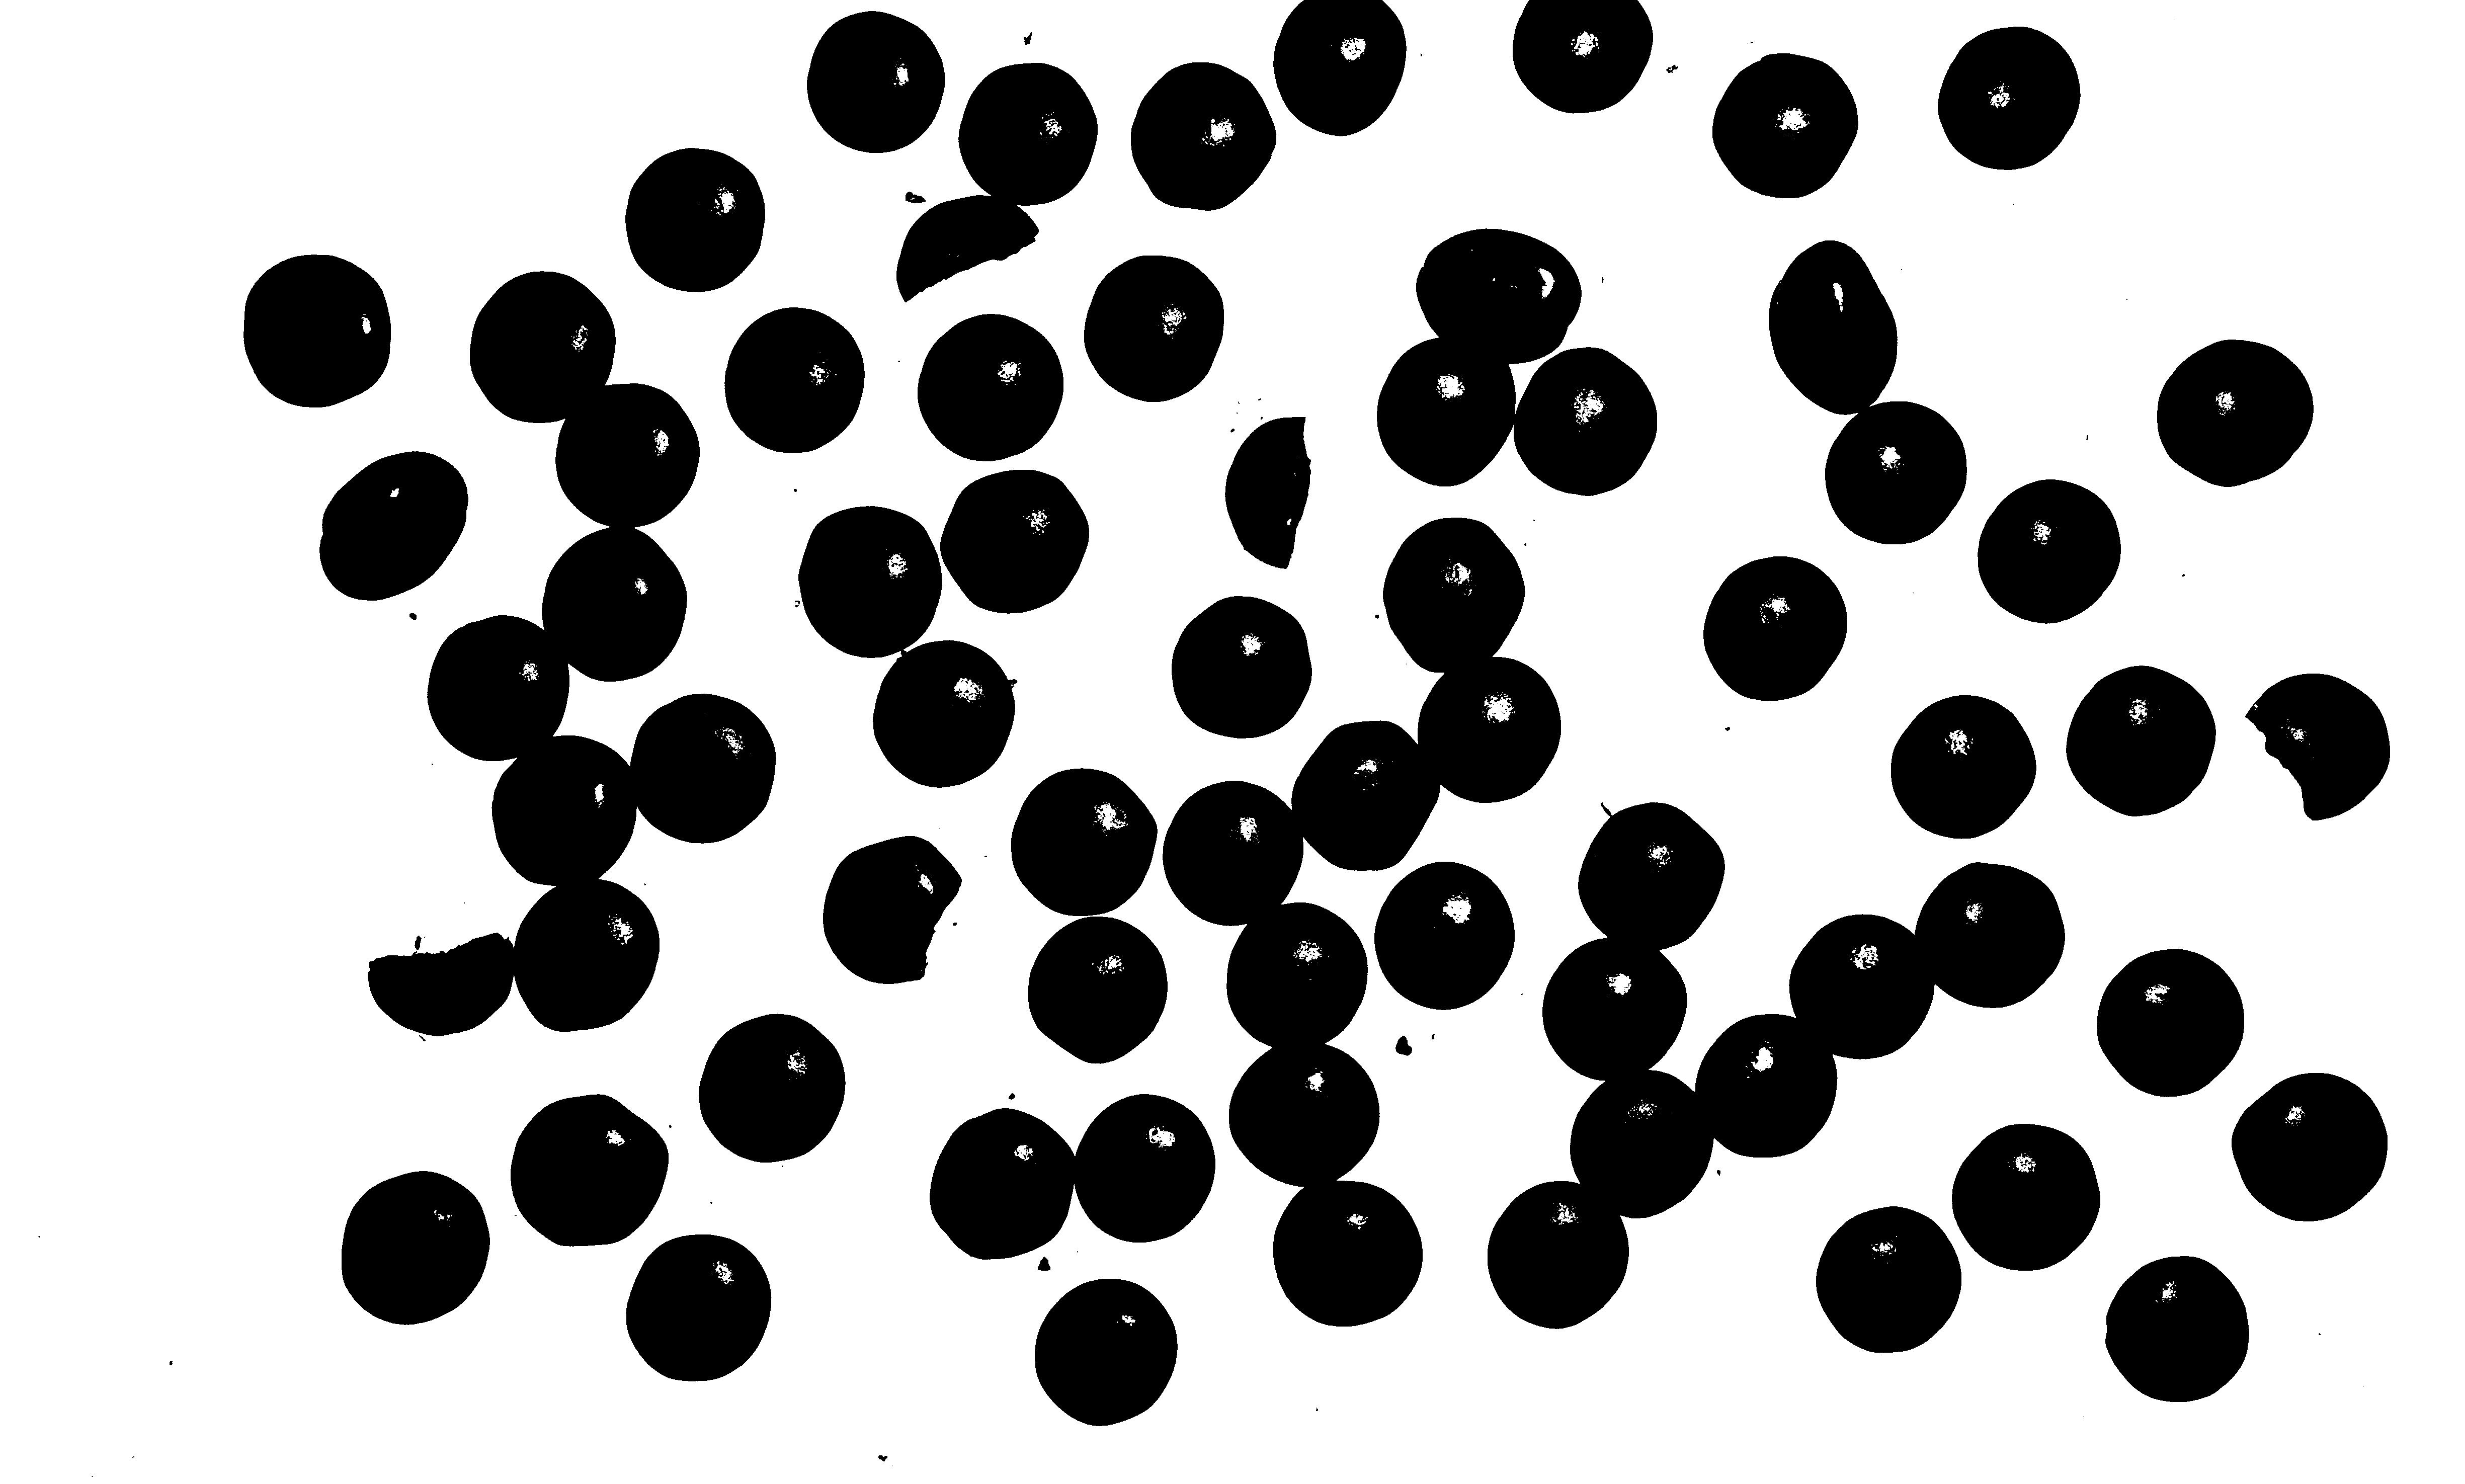
\includegraphics[width=0.7\linewidth]{pics/grey_pic_all_bin_grad}
\caption{binary treatment of Outsu-thresholding from home-made greyscale}
\label{fig:greypic2}
\end{subfigure}
\newline
\begin{subfigure}{\textwidth}
\centering
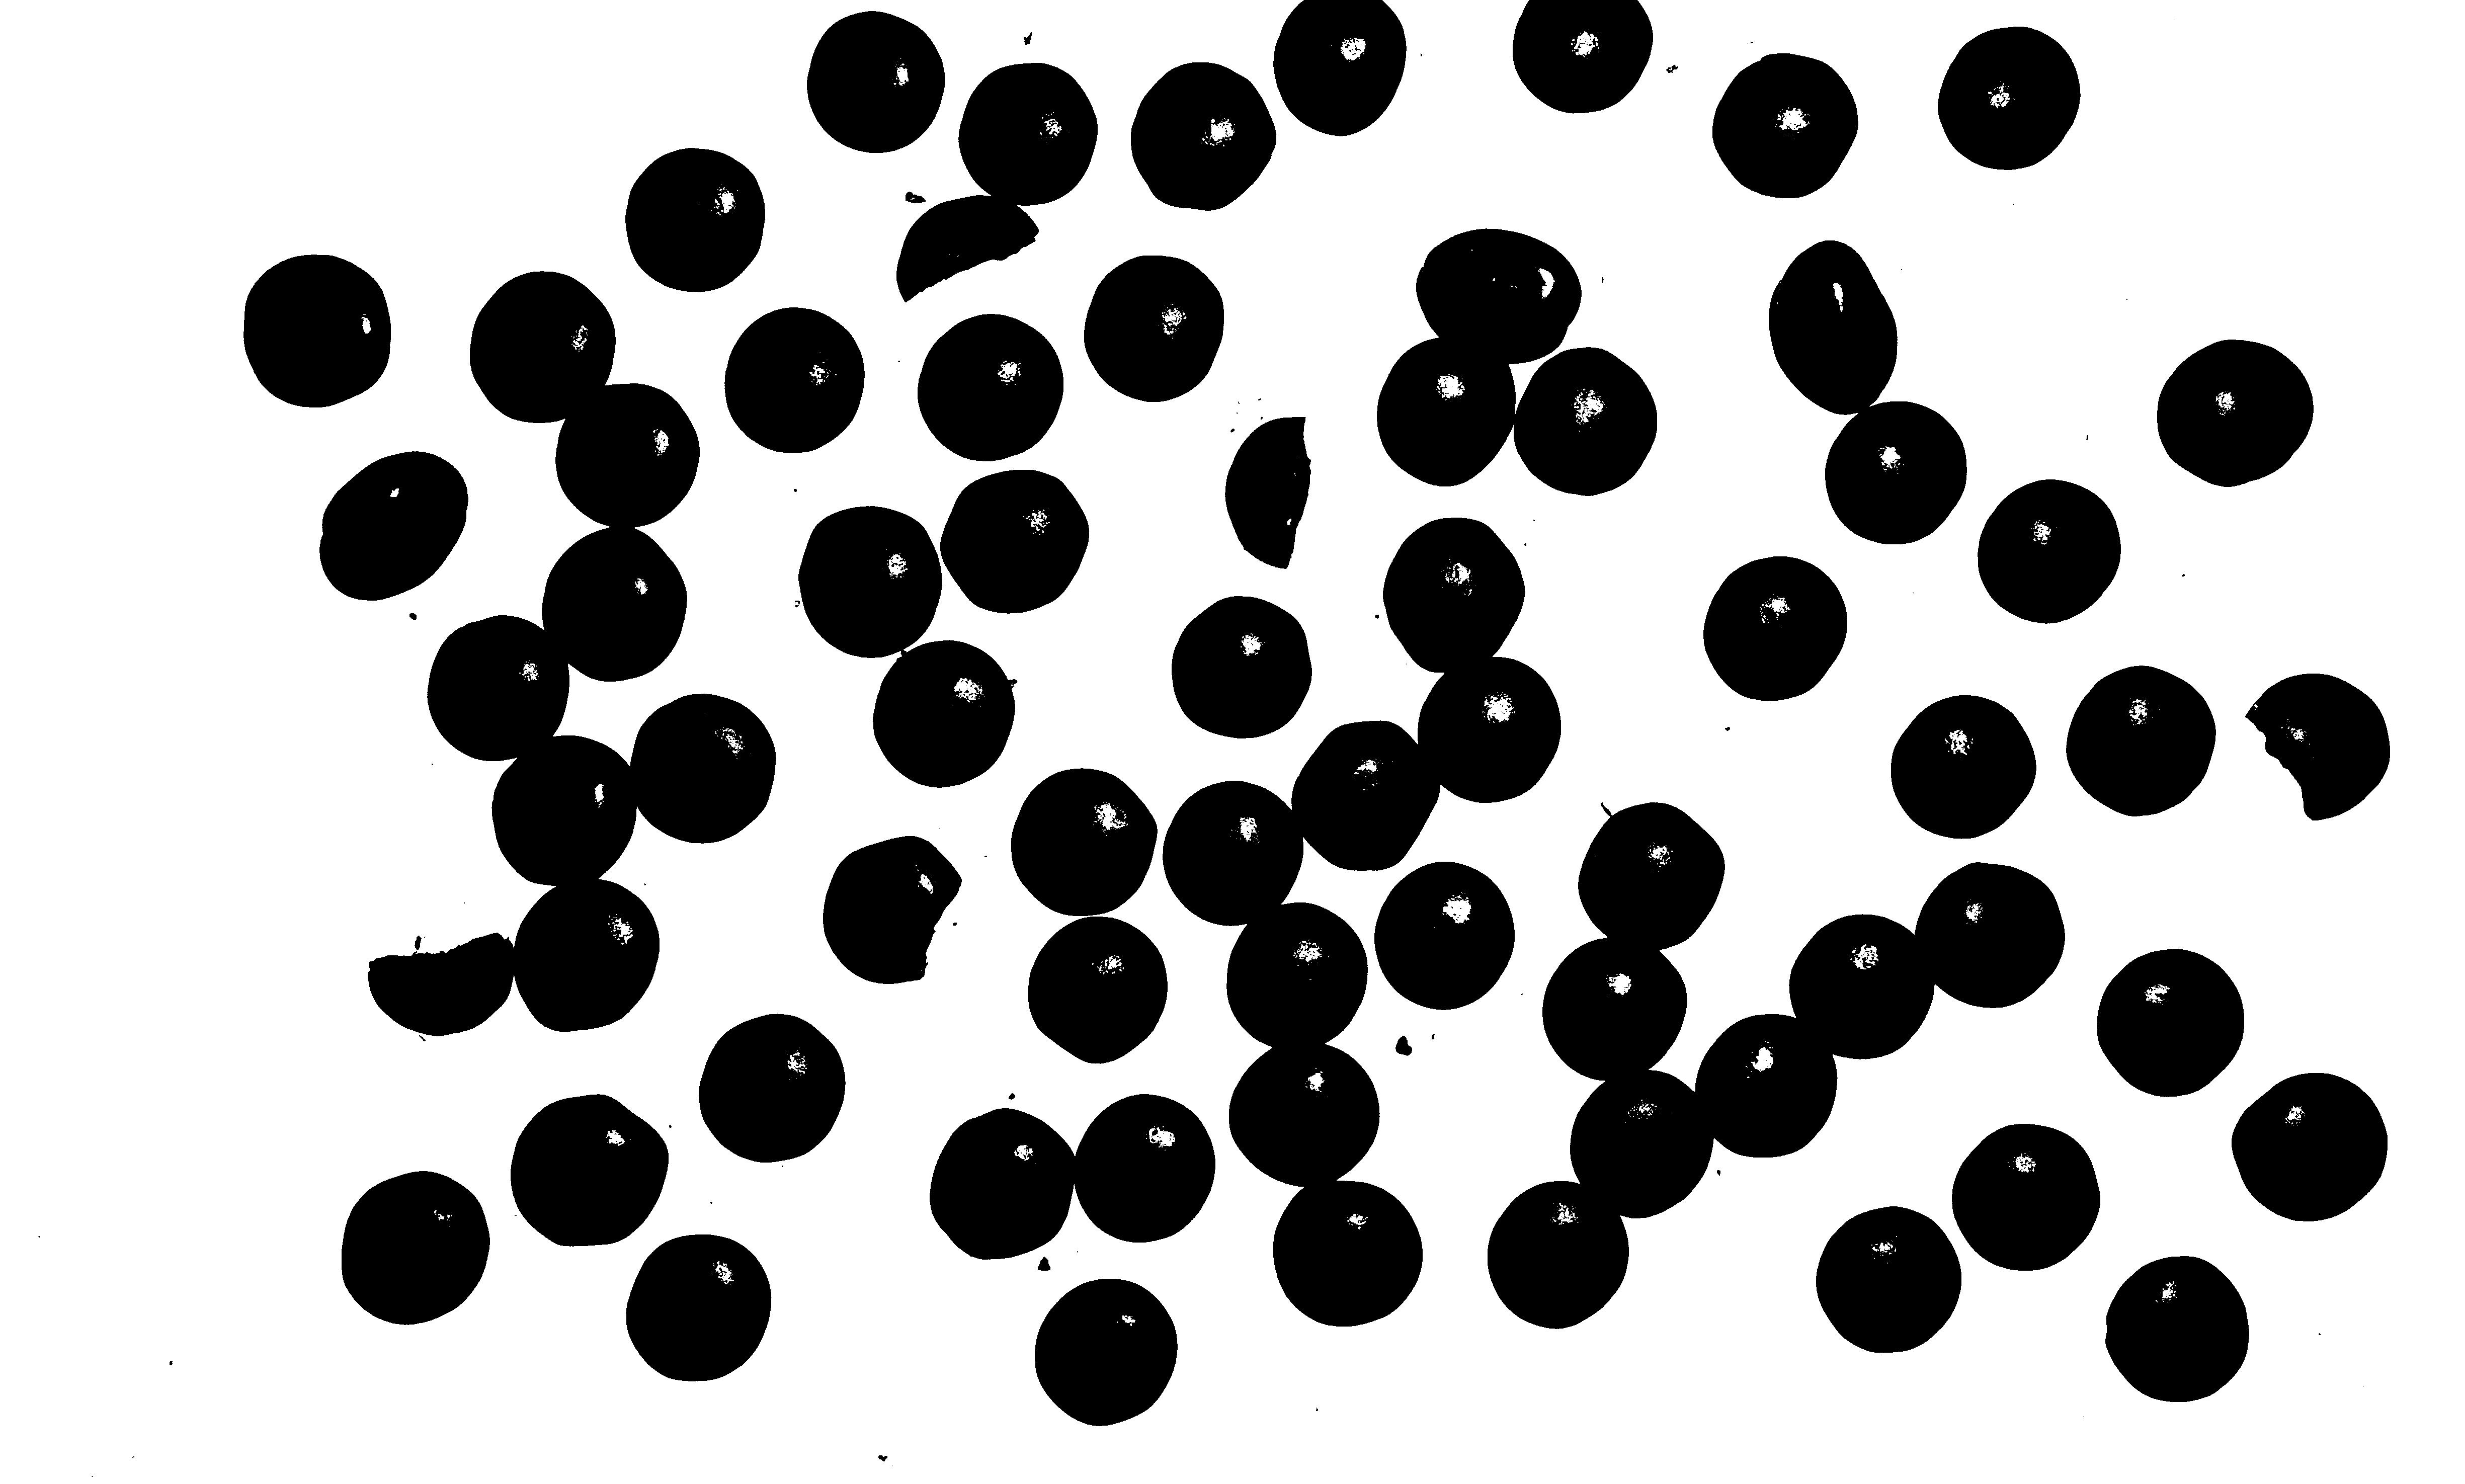
\includegraphics[width=0.7\linewidth]{pics/grey_pic_all_bin_grad}
\caption{binary treatment of Outsu-thresholding from home-made greyscale}
\label{fig:greypicallbingrad}
\end{subfigure}
\end{figure}

After that we will use "flood fill" to remove the "holes" in the picture. This step can be done with finding the contour of all figures, and then perform "flood fill" to set every pixel to appropriate values. 
What remains is to label the areas that is a individual chocolate. This can be done with Erosion, as there are some chocolates that are too close together. We will perform this until all significant particles are removed, then we dilute equal number of times with the same filter. Although this will shrink the size of the chocolate, it will not remove the centre off the chocolate which can be used to identify the location of the chocolate. Once that is done we will use Watershed to separate the last individuals into separate chocolates. Once that is done we will perform our analyses of the chocolates.

\begin{figure}[H]
\centering
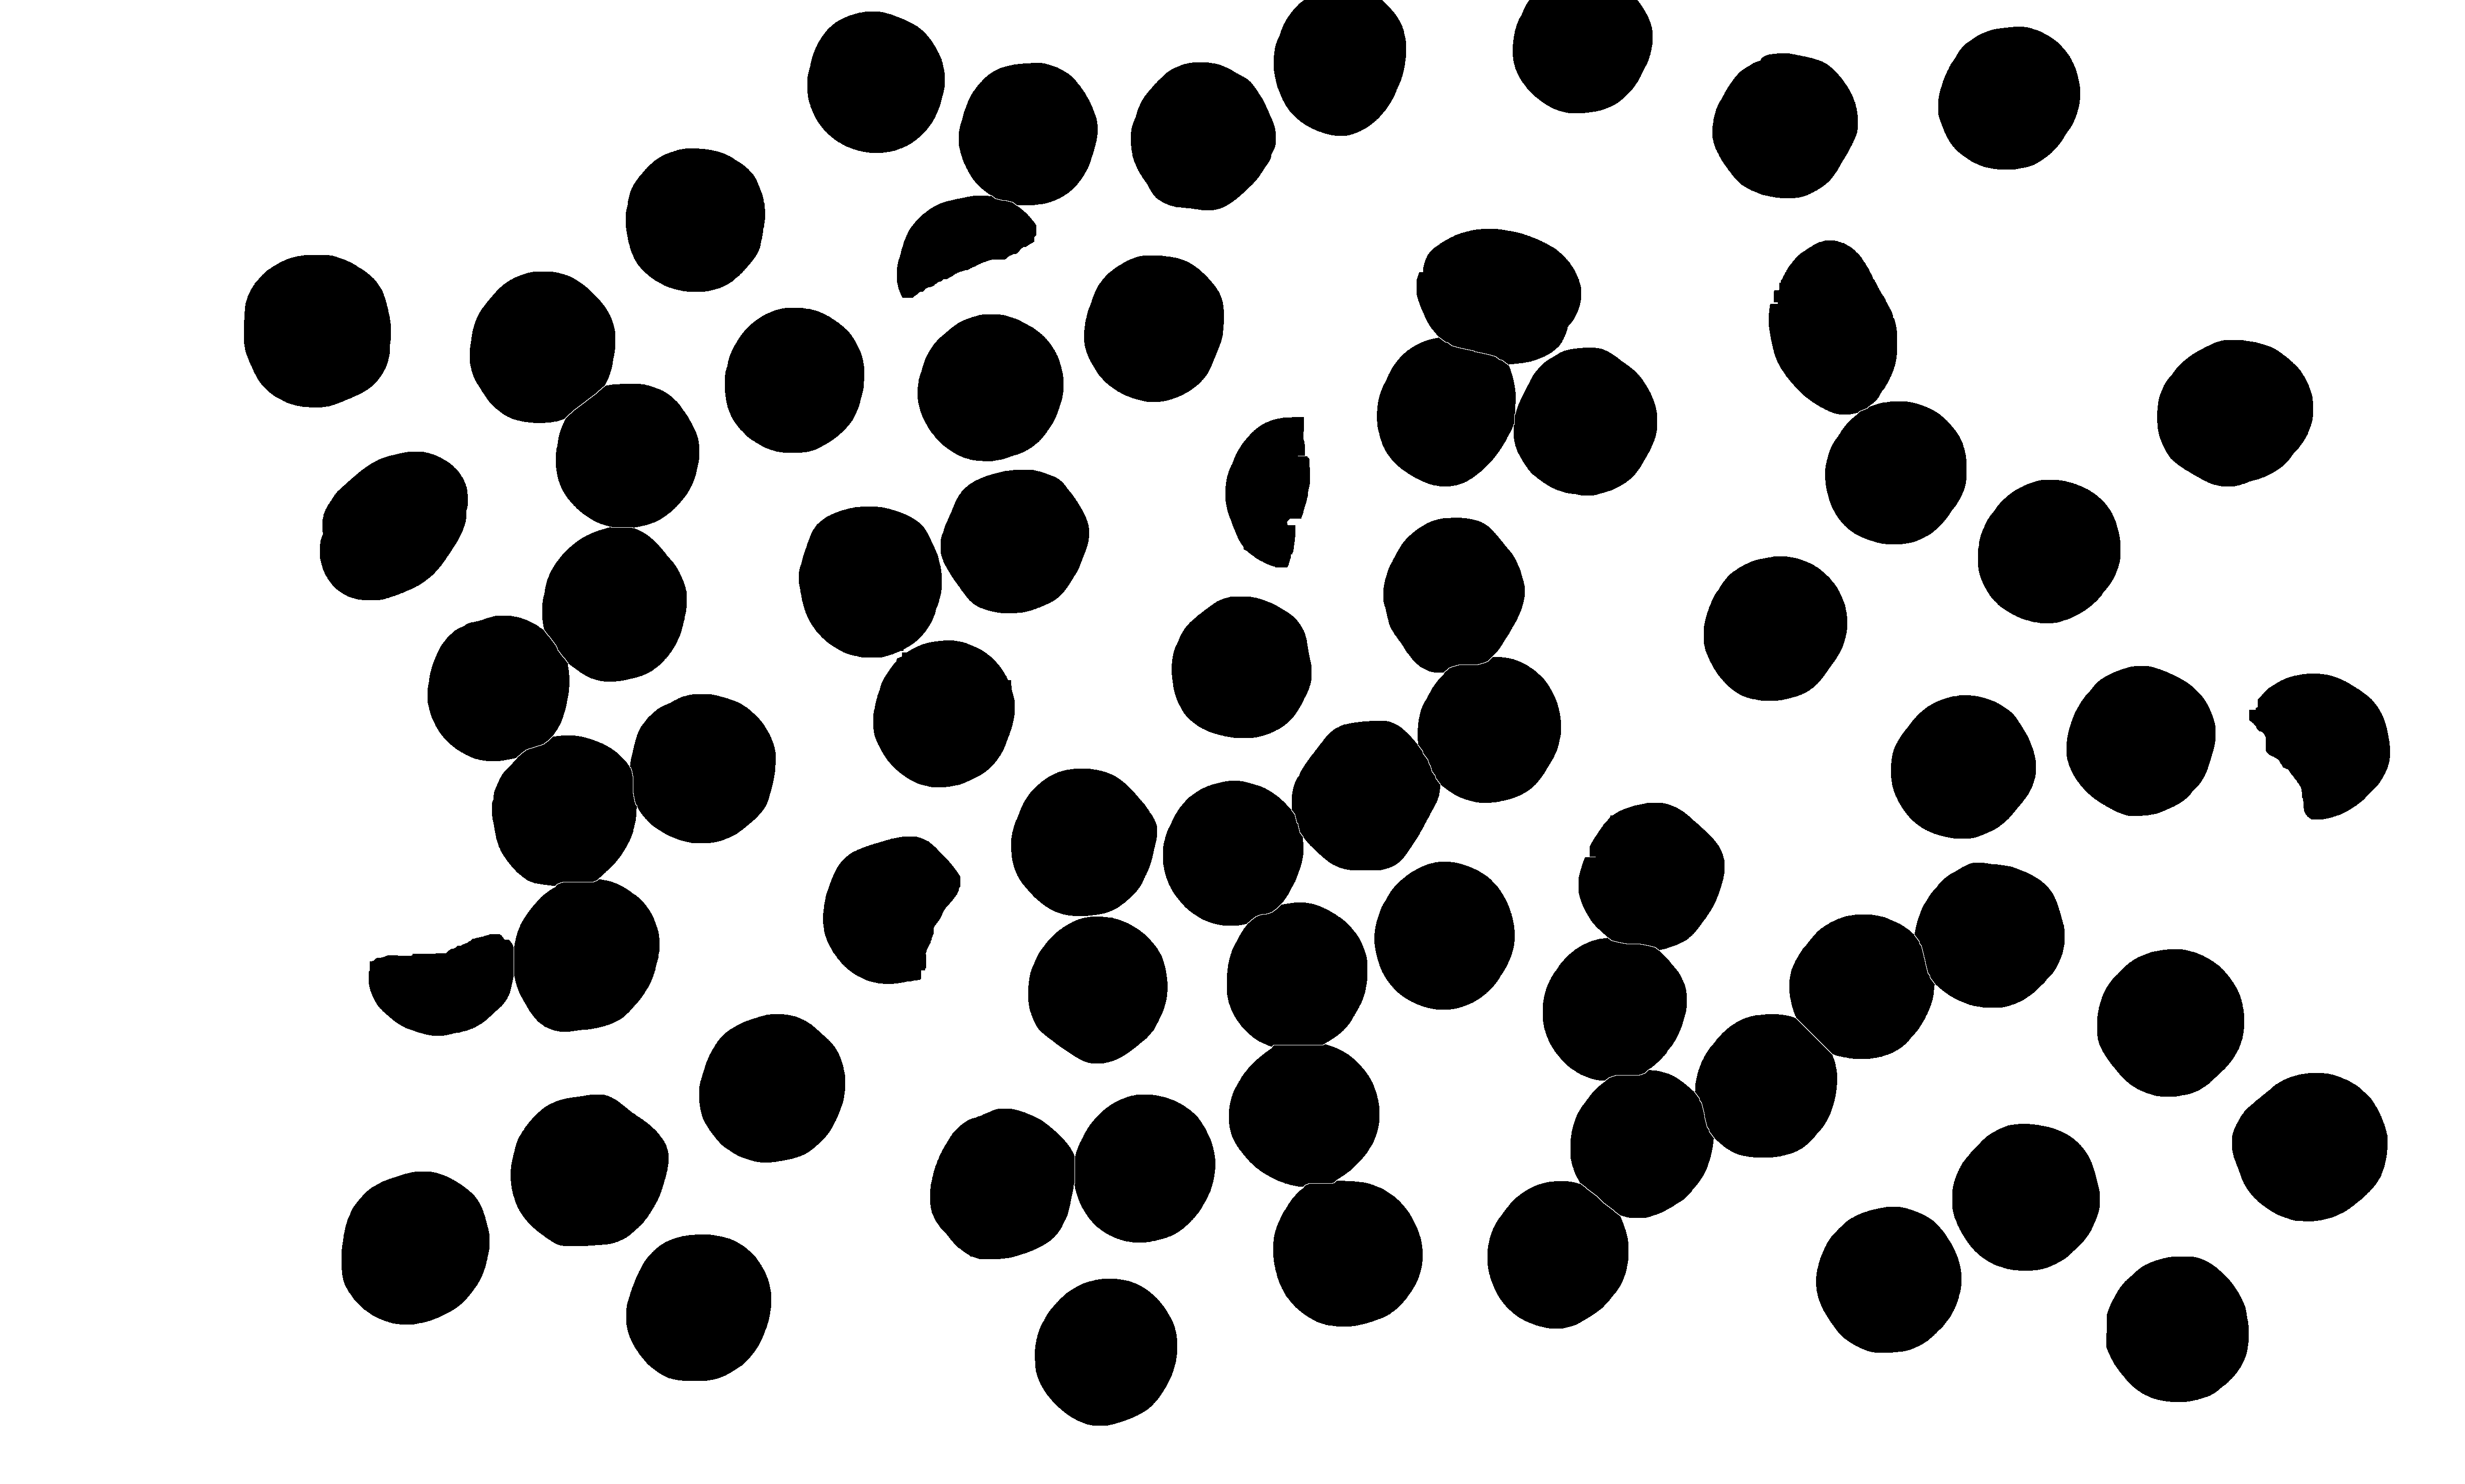
\includegraphics[width=0.7\linewidth]{pics/grey_pic_all_bin_grad_1}
\caption{Result after several erosions, and dilations. This had a side-effect of removing holes. However this could had been done by a “fill-hole” procedure.}
\label{fig:greypicallbingrad-1}
\end{figure}

When analysing the tabell generated from “analyze particles” menu we get the following table \ref{tab:imgj}
\begin{table}[H]
\centering
\begin{tabular}{|c|l|c|l|}
\hline
Label & Roundness&Label&Roundness\\\hline
1&0.930&35&0.775\\\hline
2&0.824&36&0.964\\\hline
3&0.969&37&0.949\\\hline
4&0.924&38&0.909\\\hline
5&0.949&39&0.923\\\hline
6&0.950&40&0.970\\\hline
7&0.957&41&0.952\\\hline
8&0.964&42&0.954\\\hline
9&0.500&43&0.795\\\hline
10&0.789&44&0.936\\\hline
11&0.711&45&0.988\\\hline
12&0.970&46&0.896\\\hline
13&0.934&47&0.949\\\hline
14&0.935&48&0.978\\\hline
15&0.948&49&0.953\\\hline
16&0.962&50&0.594\\\hline
17&0.944&51&0.942\\\hline
18&0.909&52&0.975\\\hline
19&0.956&53&0.949\\\hline
20&0.961&54&0.955\\\hline
21&0.944&55&0.947\\\hline
22&0.538&56&0.959\\\hline
23&0.742&57&0.940\\\hline
24&0.947&58&0.960\\\hline
25&0.938&59&0.928\\\hline
26&0.934&60&0.925\\\hline
27&0.899&61&0.971\\\hline
28&0.931&62&0.914\\\hline
29&0.928&63&0.972\\\hline
30&0.967&64&0.950\\\hline
31&0.958&65&0.977\\\hline
32&0.939&66&0.931\\\hline
33&0.962&67&0.979\\\hline
34&0.964&68&0.941\\\hline
\end{tabular}
\caption{Table extracted from ImageJ}
\label{tab:imgj}
\end{table}
The labels refers to figure \ref{fig:greypicallbingradlabel}
\begin{figure}[H]
\centering
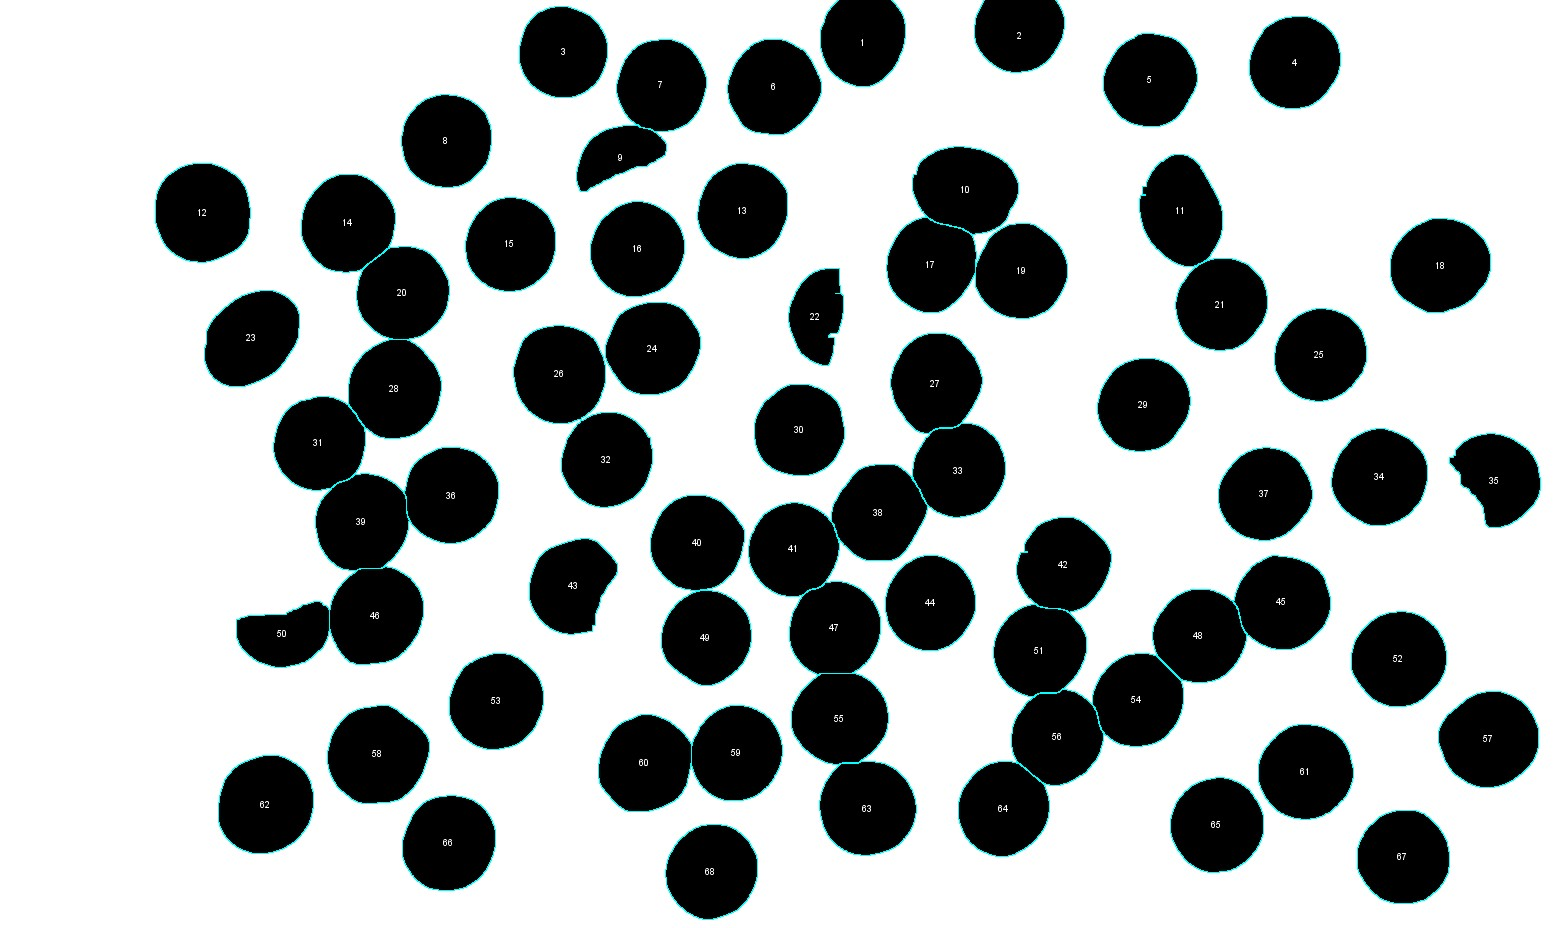
\includegraphics[width=\linewidth]{pics/grey_pic_all_bin_grad_label}
\caption{Labeled figure from imageJ}
\label{fig:greypicallbingradlabel}
\end{figure}

If we set the limit roundness to be 0.8 we find that we get the following tabel:
\begin{table}[H]
\centering
\begin{tabular}{|c|l|}
\hline
label&Roundness\\\hline
9&0.5\\\hline
10&0.789\\\hline
11&0.711\\\hline
22&0.538\\\hline
23&0.742\\\hline
35&0.775\\\hline
43&0.795\\\hline
50&0.594\\\hline
\end{tabular}
\caption{constricted table}
\label{tab:constrcted}
\end{table}

From figure \ref{fig:greypicallbingradlabel} compared with table \ref{tab:constrcted} we find this believable as we know that 10, 11, and 23 are M\&M's. The other pieces are broken pieces, some do vividly look elliptical which makes the analyses a great deal harder. The pieces in the 0.5 to 0.6 range are clearly broken Non-stop pieces.

\section{Conclusion}

From the analyses we can conclude that examinating Roundness (section \ref{eq:roundness}) we can narrow down which pieces are NoN-stop, broken NoN-stop, and M\&M's. In this case the pieces not fit for export are the pieces found in table \ref{tab:constrcted}.

\printbibliography
\end{document}

